\chapter{Theory}
\label{chap:theory}

%\epigraph{\textit{Dreaming a thought that could ~\\
%                  dream about a thought ~\\
%                  That could think of the ~\\
%                  dreamer that thought ~\\
%                  That could think of dreaming and ~\\
%                  getting a glimmer of God}
%                 }{Frank Ocean}

\section{Introduction}

The standard model (SM) of particle physics is the current best description of nature 
at its most fundamental level.
The SM incorporates the electromagnetic, weak, 
and strong forces in a single coherent framework, 
unifying the electromagnetic and weak interactions in doing so.
The SM is a type of quantum field theory known as a gauge theory, 
which represents the fundamental constituents of matter and the forces between them
as excitations of relativistic quantum fields.
Many of its predictions have been experimentally verified to unprecedented precision~\cite{PrecisionQED}.
The spontaneous breaking of gauge symmetry in the unified electroweak (EW) sector of the SM
results in the prediction of the Higgs boson \cite{HiggsPaper,BroutEnglert,KibbleEtc}, 
the existence of which is now experimentally confirmed~\cite{ATLASdiscovery,CMSdiscovery}.
In this chapter, the fundamental particles and forces of the SM are described, 
before its structure as a gauge field theory is explained.
Spontaneous symmetry breaking and its relation to the Higgs mechanism is elucidated.
The phenomenology of the Higgs boson and the consequences for experimental measurements 
are then detailed. 
Lastly, the latest precision measurements of the Higgs boson's properties are summarised 
and the simplified template cross section (STXS) framework is introduced.

\section{Fundamental particles and forces}

In the SM, particles other than the Higgs boson are divided into spin-half fermions
and spin-one bosons.
Fermions are the fundamental constituents of matter, 
and can either interact via the electromagnetic and weak forces (leptons), 
or via the electromagnetic, weak and strong forces (quarks).
Both leptons and quarks exist in three distinct generations;
the three particles comprising each family have identical properties 
except for mass, which increases across generations.
%This structure is shown in Table~\ref{tab:theory_fermions}, 
%which shows the charge and mass of each type of fermion in the SM.
In addition, each particle has a corresponding antiparticle, 
which has the same mass but whose charge and parity have the opposite sign to the original particle.

The interactions between fermions are mediated by a second class of fundamental particles, 
the gauge bosons.
Three forces are represented by the SM gauge bosons: 
the electromagnetic force, the weak force, and the strong force.
The mediator of the electromagnetic force is the massless photon, 
whilst the weak interaction occurs via the exchange of three massive particles, 
the $W^+$, $W^-$, and $Z$ bosons.
Due to the unification of these two forces into the electroweak sector of the SM, 
the photon, $W^\pm$, and $Z$ bosons arise from combinations of the fundamental gauge fields.
Gluons, which mediate the strong force, 
are massless.
%Together these describe all the fundamental forces observed in nature, 
%with the exception of gravity.
%The structure of the gauge bosons in the SM is summarised in Table~\ref{tab:theory_bosons}.

The final particle in the SM is the Higgs boson, 
which is the only scalar (spin-zero) particle in the theory.
The Higgs boson is a massive particle which arises 
due to spontaneous symmetry breaking in the electroweak sector, 
and whose existence is necessary to explain the masses of both bosons and fermions.

\section{Gauge fields}
\label{sec:theory_gauges}

The SM is realised as a particular type of quantum field theory (QFT) known as a gauge field theory.
The dynamics and predictions of a given QFT can be derived from the Lagrangian (\Like)
using the Euler-Lagrange equations, 
in the same way as the equations of motion can be derived in classical field theory~\cite{Peskin}.
Typically, a Lagrangian is constructed with the aim of respecting the symmetries 
of the physical system it is attempting to describe.
According to N\"other's theorem~\cite{Nother}, 
each symmetry of a Lagrangian has a corresponding current which is conserved.
Examples include the invariance of a Lagrangian under translations in time 
corresponding to the conservation of energy, 
and invariance under spatial translation to conservation of momentum.
The theorem therefore illustrates that the symmetries of a Lagrangian 
are intimately linked with the conserved quantities and properties of the physical system described.

The defining feature of gauge field theories is that they require the Lagrangian 
to be invariant under a local gauge transformation.
Here a local transformation means one which depends on spacetime co-ordinates, 
in contrast to a global transformation, which is constant.
Elevating a global symmetry to a local one requires the introduction of additional fields, 
which facilitate interactions between particles and imply the existence of gauge bosons.
This is illustrated below, starting with the Dirac Lagrangian 
which describes a free spin-half fermion~\cite{Dirac,Griffiths}:
\begin{equation}
\Like = i \psibar \gamma^\mu \partial_\mu \psi - m\psibar\psi ,
\end{equation}
where $\psi$ is a Dirac spinor, \psibar is its adjoint with $\psibar = \psi^\dagger \gamma^0$, 
and $\gamma^\mu$ are four $4\times4$ matrices which obey the anticommutation relation
$\{\gamma^\mu,\gamma^\nu\} = 2\Mink$ with $\Mink$ the Minkowski metric~\cite{Griffiths}.
The Dirac Lagrangian is invariant under a global phase transformation 
corresponding to the $U(1)$ group, under which the field transforms as
\begin{equation}
\psi \rightarrow e^{ig\theta} \psi ,
\end{equation}
where $\theta$ and $g$ are constant real numbers.
This invariance is dependent on the transformed field commuting with the differential operator. 
Considering instead a local gauge transformation, 
meaning the transformation is a function of the spacetime co-ordinates
\begin{equation}
\psi \rightarrow e^{ig\theta(x)} \psi , 
\end{equation}
where $\theta(x)$ now depends on the spacetime co-ordinates $x^\mu$.
The Lagrangian is no longer invariant;
instead there is a residual term remaining after the transformation
\begin{equation}
\Like \rightarrow \Like - g \psibar \gamma^\mu (\partial_\mu \theta) \psi .
\end{equation}
In order to restore gauge invariance, a new field $A^{\mu}$ can be introduced 
which transforms as
\begin{equation}
A^\mu \rightarrow A^\mu + \partial^\mu \theta
\end{equation}
This field is incorporated into the definition of the covariant derivative $D^\mu$ as
\begin{equation}
\label{eq:theory_covdev}
D^\mu = \partial^\mu + i g A^\mu , 
\end{equation}
which transforms under the local gauge transformation in the desired way
\begin{equation}
D^\mu \rightarrow e^{ig\theta(x)} D^\mu .
\end{equation}
With the addition of a free term for the field $A^\mu$, 
the form of which is constrained by the requirements of being both Lorentz and gauge invariant, 
the Lagrangian can then be written as
\begin{equation}
\label{eq:theory_EMlagrangian}
\Like = i \psibar \gamma^\mu D_\mu \psi - m\psibar\psi - \frac{1}{4} F^{\mu\nu}F_{\mu\nu},
\end{equation}
where $F^{\mu\nu} = \partial^\mu A^\nu - \partial^\nu A^\mu$.
This Lagrangian is now fully gauge invariant.
A mass term for the boson, which would take the form $m_A A_\mu A^\mu$, 
is not included since it is forbidden by local gauge invariance.
The Lagrangian in Eq.~\ref{eq:theory_EMlagrangian} 
can now be identified as a description of quantum electrodynamics (QED).
The field $A_\mu$ corresponds to a photon, and $g$ to the charge of the electron.
The interaction vertex between photons and electrons is contained in the trilinear terms
such as $\Like \supset -e \psibar \gamma^\mu A_\mu \psi$, 
and the electromagnetic field strength tensor is represented by $F^{\mu\nu}$.
This illustrates the mechanism by which local gauge invariance introduces new interacting fields
with a symmetry, in this case a $U(1)$ symmetry with one degree of freedom.
It can be shown that the number of generated bosons is equal to the number of degrees of freedom, 
or equivalently the dimension, of the symmetry group~\cite{Peskin}.
The electroweak and strong sectors of the SM follow the same principle, 
with the symmetry groups being $SU(2) \times U(1)$ and $SU(3)$ respectively.
How these symmetry transformations lead to the emergence of the desired SM properties 
is detailed in the following sections.

\subsection{Strong interactions}

The theory of strong interactions in the SM, known as quantum chromodynamics (QCD), 
is based upon the $SU(3)$ symmetry group.
The symmetries of this group can be represented by traceless $3\times3$ unitary matrices;
this implies there are eight independent matrices, or generators, of the group~\cite{Thomson}.
The covariant derivative is written as
\begin{equation}
D_\mu = \partial_\mu + i g_s \frac{\lambda^a}{2} A^a_\mu ,
\end{equation}
where $\lambda^a$ are the Gell-Mann matrices.
The eight fields $A^a_\mu$ correspond to gluons, 
the massless bosons which mediate the strong force.
The QCD equivalent of electric charge, $g_s$, is known as colour charge.
Three independent colour states exist; these are labelled red, green, and blue.
Quarks are the only SM fermions which possess colour charge, 
and thus transform as a triplet under transformations in colour space.

In addition, it should be noted that $SU(3)$ is a non-Abelian group, 
meaning that its transformations do not commute.
This introduces additional complexity to the theory, 
and has the direct consequence that gluons possess colour charge and can thus self-interact.
This is manifest in the expression for the QCD field strength tensor, given by
\begin{equation}
F^a_{\mu\nu} = \partial_\mu A^a_\nu - \partial_\nu A^a_\mu - g_s f^{abc} A^b_\mu A^c_\mu ,
\end{equation}
where  $f^{abc}$ are the antisymmetric SU(3) structure constants defined by 
$[\lambda^a,\lambda^b] = i f^{abc} \lambda^c$.
The final form of the QCD Lagrangian in the SM is then
\begin{equation}
\Like_{\textrm{QCD}} = \sum_{f} i \psibar_f (\gamma^\mu D_\mu - m_f) \psi_f 
                       - \frac{1}{4} F^a_{\mu\nu} F^{a\mu\nu} ,
\end{equation}
where the index $f$ denotes the six quark flavours and $m_f$ the quark mass of that flavour.
An important difference between QCD and QED is that the magnitude of the strong force 
increases in strength as a function of distance, rather than weakening.
Consequently particles with colour charge are never observed as free particles 
but are instead confined to colourless, composite bound states.
This is the reason quarks and gluons are detected as hadronic showers of particles, 
known as jets.

\subsection{Electroweak interactions}

One of the key successes of the SM was the unification of the electromagnetic and weak forces.
This was developed by Glashow, Weinberg and Salam~\cite{Glashow,Weinberg,Salam} 
and their GWS model constitutes the formulation of the modern SM.
Starting from the $SU(2)$ group, three fields are defined in the covariant derivative
\begin{equation}
\label{eq:theory_Wcov}
D_\mu = \partial_\mu + i \frac{g}{2} W_\mu^i \sigma^i ,
\end{equation}
where $W_\mu^i$ are the three $SU(2)$ gauge fields and $\sigma^i$ are the $2\times2$ Pauli matrices.
The corresponding charge is known as weak isospin. 
Both quarks and leptons interact via the weak interaction 
and transform as doublets under weak gauge transformations.
The weak interaction violates parity, 
meaning it is not invariant under an inversion in space co-ordinates.
This can be encoded explicitly by introducing the parity operators
\begin{equation}
P_{L,R} = \frac{1}{2} (1 \mp \gamma^5) ,
\end{equation}
where $P_{L,R}$ are the left and right handed parity operators respectively, 
and $\gamma^5 = i\gamma^0\gamma^1\gamma^2\gamma^3$, 
which anticommutes with $\gamma^\mu$ and means that objects such as $\psibar \gamma^5 \psi$
are odd under parity.
In the SM, only the left-handed fermions couple to the W bosons via $SU(2)$ interactions, 
which enables parity violation.
The formulation in Equation~\ref{eq:theory_Wcov} would suggest 
that this is true of all three $W^{\mu}$ bosons;
however it is known that the Z boson interacts with both left and right-handed fermions.
The key insight of EW unification is that the three bosons arising from the $SU(2)$ group 
can be combined with a $U(1)$ boson to form the four physically observed bosons.
This is achieved in the GWS model by constructing the $SU(2)_L \times U(1)$ group 
with weak isospin and weak hypercharge $Y$ as the respective charges, 
and $W^{i}_{\mu}$ and $B_{\mu}$ as the respective fields in the covariant derivative
\begin{equation}
\label{eq:theory_EWcov}
D_\mu = \partial_\mu + i \frac{g}{2} W_\mu^i \sigma^i + g' Y B_\mu ,
\end{equation}
with $g$ and $g'$ real numbers.
The left-handed fermions are represented by $SU(2)_L$ doublets $\psi_L$, 
whilst the right-handed fermions are singlets $\psi_R$.
The physical charged bosons are given by
\begin{equation}
W_\mu^\pm = \frac{1}{\sqrt{2}} (W_\mu^1 \mp iW_\mu^2) ,
\end{equation}
and the physical neutral bosons expressed as a rotation in the $SU(2)_L \times U(1)$ space with
\begin{equation}
\label{eq:theory_rotation}
\begin{split}
Z_\mu &= \cos{\theta_W} W_\mu^3 - \sin{\theta_W} B_\mu , \\
A_\mu &= \sin{\theta_W} W_\mu^3 + \cos{\theta_W} B_\mu ,
\end{split}
\end{equation}
where $\theta_W$ is called the Weinberg angle.
The relevant right-handed parts of the EW Lagrangian can then be written
\begin{equation}
\Like_{\textrm{EW}} \supset -\psibar_R g' \cos{\theta_W} Y_\psi \gamma^\mu A_\mu \psi_R .
\end{equation}
By comparison with the electromagnetic Lagrangian, 
the relation $g' \cos{\theta_W} = |e|$ for the magnitude of the electron charge can be inferred.
The hypercharge $Y_\psi$ is identified as the value of the particle's electric charge.
Finally, the left-handed terms include
\begin{equation}
\Like_{\textrm{EW}} \supset - \psibar_L(g\sin{\theta_W} \frac{\sigma^3}{2} 
                            + g' \cos{\theta_W} Y_\psi) \gamma^\mu A_\mu \psi_L .
\end{equation}
In order for the doublets representing the quarks and leptons to have charges 
which differ by one unit of charge, it is inferred that $g\sin{\theta_W} = e$. 
The hypercharges of the quarks and leptons are then required to be 
$+\frac{1}{6}$ and $-\frac{1}{2}$ respectively.
The theory thus describes a photon which couples in the same way to left and right-handed fields, 
whilst allowing the weak interaction to violate parity, exactly as observed in nature. 

This completes the description of how fermions and bosons interact in the SM.
However an issue remains relating to the particle masses.
As was described in Section~\ref{sec:theory_gauges}, 
mass terms for the bosons are not invariant under local gauge transformations.
This is not an issue for the description of the photon, 
but cannot be reconciled with the experimentally observed finite masses of the W and Z bosons.
Furthermore, it can be seen that a mass term of the form
\begin{equation}
\label{eq:theory_badmass}
\Like_{\textrm{mass}} = -m(\psibar_L \psi_R + \psibar_R \psi_L)
\end{equation}
is not gauge invariant, since the left and right-handed spinors transform in different ways.
These considerations prevent the inclusion of mass terms 
for the quarks and leptons in the Lagrangian.
Spontaneous symmetry breaking and the Higgs mechanism provide the resolution to this problem.

\section{Spontaneous symmetry breaking}

The SM grants masses to the W and Z bosons via spontaneous symmetry breaking 
in the EW sector.
This is known as the Higgs mechanism, 
which was conceived concurrently by several people 
during the 1960s~\cite{HiggsPaper,BroutEnglert,KibbleEtc}.
The mechanism can be illustrated using the Lagrangian 
for a locally gauge invariant complex scalar field $\phi$ 
with a fourth-order interaction term~\cite{Thomson}
\begin{equation}
\label{eq:theory_SSMlagrangian}
\Like = (D^\mu \phi^*) (D_\mu \phi) - m^2 \phi^*\phi 
        - \lambda (\phi^*\phi)^2 - \frac{1}{4} F^{\mu\nu}F_{\mu\nu} ,
\end{equation}
where $\lambda$ is a positive real constant %check that I understand the difference between global and local here
and the covariant derivative is as defined in Equation~\ref{eq:theory_covdev}.
Provided the $m^2$ term is positive, this potential has its minimum at $\phi=0$.
However the introduction of the quartic term permits the $m^2$ term to be negative, 
which results in a degenerate set of minima at non-zero values
\begin{equation}
|\phi| = \frac{\sqrt{-m^2}}{2\lambda} \equiv \frac{v}{\sqrt{2}} ,
\end{equation}
where the vacuum expectation value $v$ has been defined.
Although the potential itself is symmetric, the physical vacuum state is not;
this is what is meant by the term spontaneous symmetry breaking.
The shape of this potential is illustrated in Figure~\ref{fig:theory_SSB}.

\begin{figure}[hptb]
  \centering
  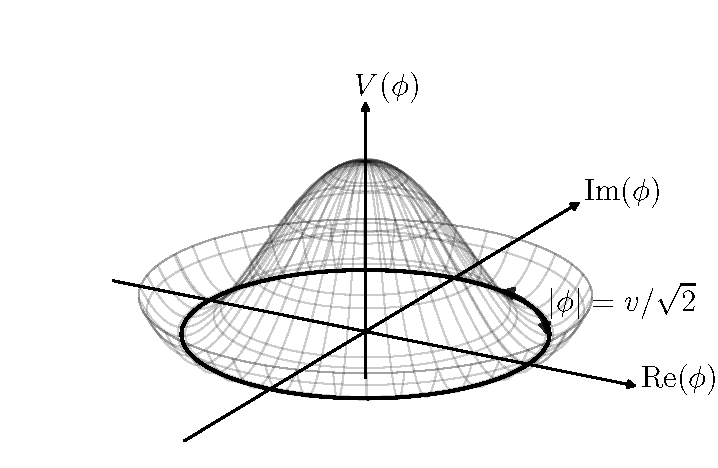
\includegraphics[width=0.7\textwidth]{Figures/Theory/SSB.pdf}
  \caption[Quartic potential exhibiting spontaneous symmetry breaking.]
  {
    The shape of the quartic potential described in Equation~\ref{eq:theory_SSMlagrangian}.
    The potential itself is symmetric, 
    but the symmetry is broken when a specific choice of ground state is made 
    from the degenerate set of available minima.
  }
  \label{fig:theory_SSB}
\end{figure}

Making the arbitrary choice of the ground state being in the real direction, 
it is possible to expand about the minimum with a field of the form
\begin{equation}
\phi = \frac{1}{\sqrt{2}} (v + \phi_1 + i\phi_2) ,
\end{equation}
where $\phi_1$ and $\phi_2$ are real scalar fields.
Substituting this into the Lagrangian (Equation~\ref{eq:theory_SSMlagrangian}) yields the mass terms
\begin{equation}
\Like \supset - 2 \lambda v^2 \phi^2_1 + 2 g^2 v^2 A^\mu A_\mu .
\end{equation}
Thus the gauge boson $A_\mu$ has acquired mass;
spontaneous symmetry breaking of a Lagrangian invariant under local gauge transformations 
yields a massive gauge boson. 
This important result underlies the generation of masses for the SM vector bosons.
Furthermore, there is now an additional massive scalar particle $\phi_1$;
this will shortly be identified as the Higgs boson.

In the SM, the scalar Higgs field transforms as an $SU(2)$ doublet $H$ 
which has the required four degrees of freedom. 
Its potential is fourth order such that the Lagrangian can be written 
\begin{equation}
\Like_{\textrm{EW}} \supset (D^\mu H)^\dagger (D_\mu H) + \mu^2 H^\dagger H - \lambda (H^\dagger H)^2 ,
\end{equation}
where $\mu$ and $\lambda$ are positive constants 
and the covariant derivative is as defined in Equation~\ref{eq:theory_EWcov}.
This potential also has a degenerate set of non-zero minima with 
\begin{equation}
H^\dagger H = \frac{\mu^2}{2\lambda} \equiv \frac{v^2}{2} , 
\end{equation}
and the choice can be made to expand about the minimum 
in the neutral component of the doublet such that 
\begin{equation}
H = \left(
\begin{split}
&0 \\
\frac{v}{\sqrt{2}} &+ h(x)
\end{split}
\right) ,
\end{equation}
where $h(x)$ is the physical scalar field of the theory.
Parameterising the field in this way corresponds to choosing the unitary gauge.
The covariant derivative acting on the Higgs field then results in, 
after the rotation described in Equation~\ref{eq:theory_rotation}, the Lagrangian terms
\begin{equation}
\Like_{\textrm{EW}} \supset \frac{g^2v^2}{4} W^+_\mu W^{-\mu} 
                         + \frac{(g^2 + g^{\prime 2})v^2}{8} Z_\mu Z^\mu .
\end{equation}
Thus the W and Z bosons have acquired mass whilst leaving the photon massless.
The Higgs mechanism is therefore able to explain the observed mass structure of the gauge bosons.
Furthermore, the ratio of the masses of the and W and Z bosons 
is predicted to be equal to $\cos{\theta_W}$, which is also in agreement with experiment.
This pattern of symmetry breaking depends on 
the choice of direction for the vacuum expectation value and Higgs field;
it has been chosen by construction to match the observed SM bosons and fermions. %e.g. the cos(theta) relations would change if chose different gauge/direction

In addition to explaining the masses of the gauge bosons, 
the Higgs mechanism enables mass terms for the fermions to be included in the Lagrangian.
These terms are known as Yukawa terms~\cite{Thomson}
\begin{equation}
\Like_{\textrm{EW}} \supset \frac{g_f}{\sqrt{2}} v \psibar_L H \psi_R + h.c.~,
\end{equation}
where $g_f$ is the Yukawa coupling of the fermion to the Higgs boson 
and $h.c.$ indicates the Hermitian conjugate.
This combination is now gauge invariant, 
in contrast to the mass terms in Equation~\ref{eq:theory_badmass}.
Expanding the field $H$ in terms of the vacuum expectation value and the field $h(x)$, 
the mass terms generated for the fermions are 
\begin{equation}
m_f = \frac{g_f v}{\sqrt{2}}
\end{equation}
The magnitude of the Yukawa coupling is not known a priori and must be measured experimentally.
It can then be seen that there are also interactions between the fermions and the Higgs boson
whose coupling strength is proportional to the fermion mass, as well as the Higgs boson mass. %reference to three generations and CKM matrix?

Furthermore, the Higgs boson also has interaction terms with the gauge bosons.
The relevant terms in the Lagrangian are
\begin{equation}
\Like_{\textrm{EW}} \supset m_W^2 \left( \frac{2h}{v} + \frac{h^2}{v^2} \right) W^+_\mu W^{-\mu}
                 + \frac{m_Z^2}{2} \left( \frac{2h}{v} + \frac{h^2}{v^2} Z_\mu Z^{\mu} \right),
\end{equation}
which describe the three point and four point interactions between the massive gauge bosons 
and the Higgs boson.
Again the coupling strength is proportional to both the gauge boson mass and the Higgs boson mass.
The Higgs boson mass terms in the Lagrangian together with its self-interactions are 
\begin{equation}
\Like_{\textrm{EW}} \supset - \lambda v^2 h^2 - \lambda v h^3 - \frac{1}{4} \lambda h^4 ,
\end{equation}
where the Higgs boson mass can now be identified as $m_H = \sqrt{2\lambda}v$.
The mass itself is unknown a priori, and must be measured experimentally.
Given the Higgs boson mass, and considering all these interaction terms involving the Higgs boson, 
it is possible to infer the phenomenology of how the Higgs boson is produced and how it decays.
This phenomenology and its consequences for experimental measurements 
of the Higgs boson's properties are discussed in the following section.

\section{Properties of the Higgs boson}

Discovering the Higgs boson, and thereby reaching observation of all elements of the standard model, 
was one of the main physics objectives of the LHC. %revise LEP & Tev constraints
This goal was achieved in 2012 when both the ATLAS and CMS experiments 
announced the discovery of a new particle resembling the Higgs boson~\cite{ATLASdiscovery,CMSdiscovery}.
Several Higgs boson production modes and decay channels were analysed.
Now that the existence of the Higgs boson is confirmed, 
the experimental focus is to measure its properties as precisely as possible.
This enables stringent tests of the SM to be made, 
and in so doing either observe discrepancies from its predictions
which indicate the presence of physics beyond the standard model (BSM), 
or place constraints on the permitted form of possible BSM theories.
In this section the most important production and decay modes for Higgs boson measurements
at the LHC are described, and current state-of-the-art results are summarised.

\subsection{Higgs boson production at the LHC}

The LHC produces high energy collisions between two circulating beams of protons.
The production of the Higgs boson can be initiated in different ways, 
with cross sections that depend on the centre-of-mass energy (\sqrtS) of the proton-proton collision
and the Higgs boson mass.
For collisions at $\sqrtS=\SI{13}{TeV}$ and a Higgs boson mass of around \SI{125}{GeV}, 
gluon fusion (ggH) is the dominant mode~\cite{YR4}.
The ggH final state contains only the Higgs boson. 
This contrasts with other modes, such as vector boson fusion (VBF), 
which produces a Higgs boson together with two quarks that hadronise to form jets.
These additional objects can improve the ability to discriminate the Higgs boson signal 
from background, meaning events which have similar detector signatures to the Higgs boson
but arise from other SM processes.
Other important production modes whose existence has been confirmed at the LHC include 
vector boson-associated production (VH) 
and production in association with a top quark-antiquark pair (ttH).
Figure~\ref{fig:theory_FeynProd} shows the leading order Feynman diagrams 
for these four production modes, showing explicitly the additional objects present 
in events produced by modes other than ggH.
The expected SM cross sections for each process, and for the rarer tH and bbH processes, 
are shown in Table~\ref{tab:theory_prod}.
Experimental sensitivity to a given process depends not only on the signal cross section 
but also the amount of background.
Observations of the ggH and VBF were made during Run 1 
of the LHC~\cite{ATLAScouplingsRun1,CMScouplingsRun1,ATLASandCMScouplingsRun1}, 
with the VH and ttH modes being observed more recently 
using Run 2 data~\cite{ATLASttHobservation,CMSttHobservation,ATLASbbObservation,CMSbbObservation}.

\begin{table}
  \centering
  \begin{tabular}{ l | c c c c c c c }
      \hline
      Production mode & ggH & VBF & WH & ZH & ttH & bbH & tH  \\
      \hline
      Cross section (pb) & 48.71 & 3.78 & 1.37 & 0.88 & 0.51 & 0.49 & 0.07 \\
      \hline
  \end{tabular}%} 
  \caption[Cross sections of the main Higgs boson production processes.]
  {
    Cross section values for the main Higgs boson production processes at the LHC, 
    for $\sqrt{s}=\SI{13}{TeV}$ and $m_H = \SI{125}{GeV}$.
    Values are taken from Ref.~\cite{YR4}.
  }
  \label{tab:theory_prod}
\end{table}

\begin{figure}[hptb]
  \centering
  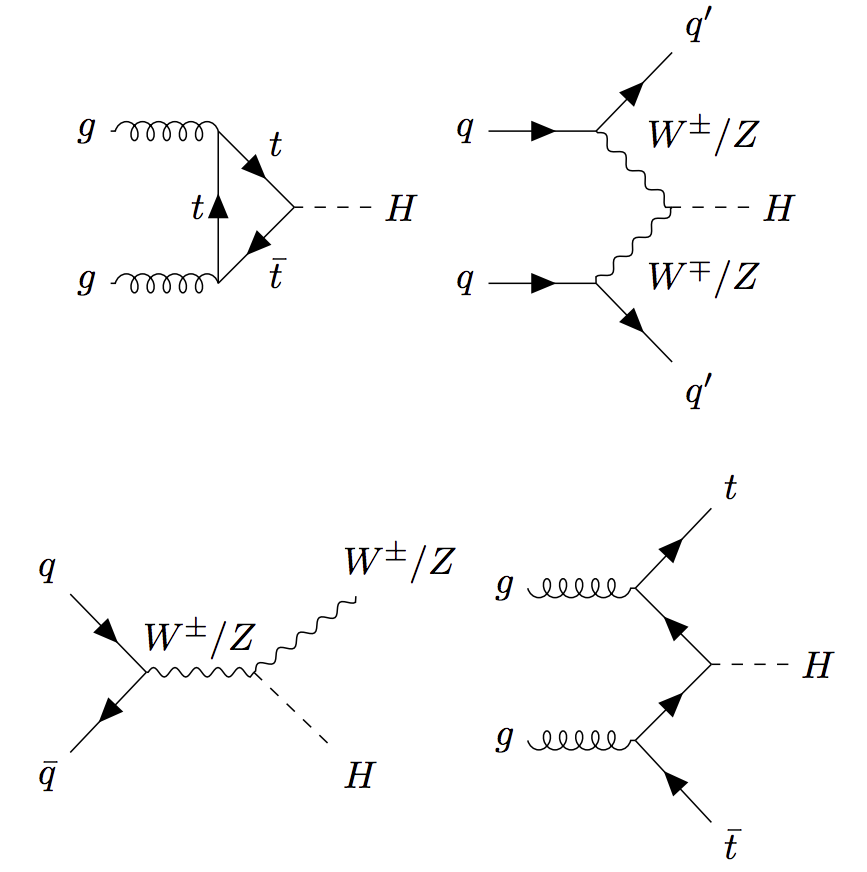
\includegraphics[width=0.7\textwidth]{Figures/Theory/FeynProd.png}
  \caption[Feynman diagrams of four Higgs boson production modes.]
  {
    Feynman diagrams representing the four principal Higgs boson production modes at the LHC.
    In descending order of cross section, these are: ggH in the top left, VBF in the top right, 
    VH in the bottom left, and ttH in the bottom right.
  }
  \label{fig:theory_FeynProd}
\end{figure}

\subsection{Higgs boson decay modes}

The SM predicts that the Higgs boson has an extremely short lifetime~\cite{YR4}.
The Higgs boson is therefore never observed directly, 
but instead its presence is inferred from its decay products.
There are several permitted decay modes of the Higgs boson.
Since its coupling strength to other particles is proportional to the mass of the decay product, 
it can decay directly to any massive particle\footnote{Only decays to pairs of particles 
whose mass is less than half that of the Higgs boson are permitted kinematically. 
However the decay can still occur to virtual particles of greater mass, which then themselves decay.}.
In addition, loop diagrams permit the decay to massless particles, including the gluon and photon.
The branching fractions for each of the seven principal decay modes 
is shown in Table~\ref{tab:theory_decay}.
Observations of the $\gamma\gamma$, $\mathrm{ZZ}^{*}$, $W^{\pm}W^{\mp*}$, 
and $\tau^+\tau^-$ decay modes were made during Run 1 
of the LHC~\cite{ATLAScouplingsRun1,CMScouplingsRun1,ATLASandCMScouplingsRun1}, 
with the $b\bar{b}$ mode being observed more recently 
using Run 2 data~\cite{ATLAStautauObservation,CMStautauObservation,ATLASbbObservation,CMSbbObservation}.

\begin{table}
  \centering
  \begin{tabular}{ l | c c c c c c c }
      \hline
      Decay mode & $b\bar{b}$ & $W^{\pm}W^{\mp*}$ & $gg$ & $\tau^+\tau^-$ & $c\bar{c}$ & $\mathrm{ZZ}^{*}$ & $\gamma\gamma$ \\
      \hline
      Branching fraction & 58.2\% & 21.4\% & 8.2\% & 6.3\% & 2.8\% & 2.6\% & 0.23\% \\
      \hline
  \end{tabular}%} 
  \caption[Branching fractions of the main Higgs boson decay modes.]
  {
    Branching fractions of the main Higgs boson decay modes. 
    Values are taken from Ref.~\cite{YR4}.
  }
  \label{tab:theory_decay}
\end{table}

It can be seen that the decay to $b\bar{b}$ has the largest branching fraction.
However due to the large hadronic background at the LHC, 
this decay channel is very difficult to utilise experimentally.
The channels with the greatest sensitivity, despite their relatively low branching fractions, 
are the diphoton ($\gamma\gamma$) and $ZZ^{*}$ decays 
(where $Z^{*}$ indicates a virtual, or off mass-shell, Z boson).
The sensitivity of these channels depends on the relatively low background 
and the ability to precisely reconstruct the mass of the Higgs boson from the decay products.
The analyses of the $\gamma\gamma$ and $ZZ^{*}$ decay channels were the most important 
at the time of the discovery of the Higgs boson, 
and for the same reasons are now are ideally suited to the study of its properties.
This analysis uses the diphoton decay channel.
Three Feynman diagrams representing the largest contributions to the effective vertex 
between the Higgs boson and two photons are shown in Figure~\ref{fig:theory_FeynDecay}.
As can be seen in the figure, 
the decay to two photons is therefore sensitive to the Higgs boson's coupling to other particles, 
including the top quark and the W boson.

\begin{figure}[hptb]
  \centering
  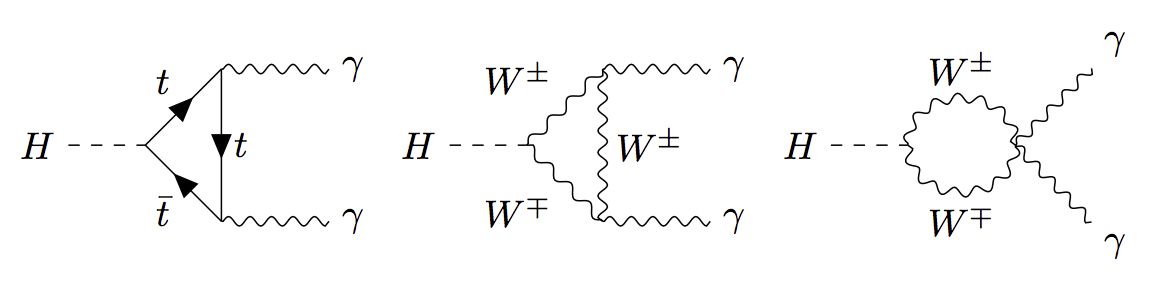
\includegraphics[width=\textwidth]{Figures/Theory/FeynDecay.png}
  \caption[Feynman diagrams contributing to the \Hgg decay loop.]
  {
    The Feynman diagrams with the largest contribution to the \Hgg decay loop.
    The diagrams involving the top quark have opposite sign to those involving the W boson, 
    leading to destructive interference.
  }
  \label{fig:theory_FeynDecay}
\end{figure}

\subsection{Status of Higgs boson measurements}

Since its discovery, remarkable progress has been made 
in measuring the properties of the Higgs boson.
Several aspects of the SM Higgs boson structure can be tested experimentally.
The first is the spin of the Higgs boson; it is the only fundamental scalar particle within the SM.
Due to the observed decay to two spin-one photons, the Higgs boson must have even spin.
Dedicated measurements by ATLAS and CMS have excluded both the spin-two hypothesis 
and the hypothesis of a Higgs boson with zero spin
but negative parity (a pseudoscalar)~\cite{ATLASspinHiggs,CMSspinHiggs}. %TODO understand what goes on here
The possibility that the observed Higgs boson is a mixture of scalar 
and pseudoscalar states has not been ruled out, and remains an active subject of research.

Furthermore, the mass of the Higgs boson has also been measured precisely. 
The $\gamma\gamma$ and $\mathrm{ZZ}^{*}$ modes are the two decay channels with sufficiently narrow 
mass resolution to contribute to this measurement.
During Run 1, the combination of ATLAS and CMS analyses led to the measurement of the Higgs boson 
mass to be $\mH = 125.09 \pm \SI{0.24}{GeV}$~\cite{ATLASandCMSmass}.
This has since been superseded by the measurements made by CMS in the $\mathrm{ZZ}^{*}$ channel 
with Run 2 data, where a precision of better than 0.2\%~\cite{HIG-16-041} is obtained.
The observed value and its uncertainty is $\mH = 125.26 \pm \SI{0.21}{GeV}$.

The coupling of the Higgs boson to other SM particles can also be measured experimentally, 
by comparing the rate of Higgs boson production to the expectation from the SM.
These measurements can be parameterised in different ways.
For results based on Run 1 data, two different schemes were commonly used.
The first utilises signal strength modifiers $\mu$, 
which are defined as the ratio of the observed Higgs boson yield to the SM expectation.
This can be defined inclusively, for all Higgs boson production and decay modes, 
or for individual combinations of production and decay modes.
The general definition is written as
\begin{equation}
\mu^f_i = \frac{\sigma_i\mathcal{B}^f}{(\sigma_i)_{\textrm{SM}}(\mathcal{B}^f)_{\textrm{SM}}} ,
\end{equation}
where $\sigma_i$ and $\mathcal{B}^f$ are the observed production cross section 
and decay branching fraction respectively, 
and the ``SM" subscript refers to their respective SM predictions.
The second is the so-called $\kappa$-framework~\cite{YR3}, 
which is motivated by the leading-order couplings of the Higgs boson to bosons and fermions.
The coupling modifiers $\kappa_j$ are defined such that 
\begin{equation}
\kappa^2_j = \frac{\sigma_j}{\sigma_j^{\textrm{SM}}} \; \mathrm{or} \; \frac{\Gamma_j}{\Gamma_j^{\textrm{SM}}} ,
\end{equation}
where in the SM the values of all the $\kappa_j$ are equal to unity.
In addition to including couplings to individual particles or groups of particles, 
effective coupling modifiers $\kappa_g$ and $\kappa_\gamma$, 
which describe the loop processes of ggH production and diphoton decay respectively, can be defined.
The combination of ATLAS and CMS Run 1 analysis documented in Ref.~\cite{ATLASandCMScouplingsRun1} 
presents results in terms of both signal strength modifiers and coupling modifiers.

An example of signal strength modifier measurements 
from the previous CMS ${\Hgg}$ analysis \cite{HIG-16-040} is shown in Figure~\ref{fig:theory_PerProcTrad}.
The modifiers for the ggH, VBF, ttH and VH production processes and the diphoton decay are shown, 
with the inclusive diphoton decay modifier overlaid.
In this single decay channel with one experiment, 
the ggH signal strength is already measured to a precision of 20\%.
Combinations of results across different decay channels performed for optimal precision,
with the inclusive Higgs boson signal strength now measured 
to a precision of around 10\%~\cite{ATLAScomb,CMScomb}.
So far, all measurements are consistent with the SM predictions.

\begin{figure}[hptb]
  \centering
  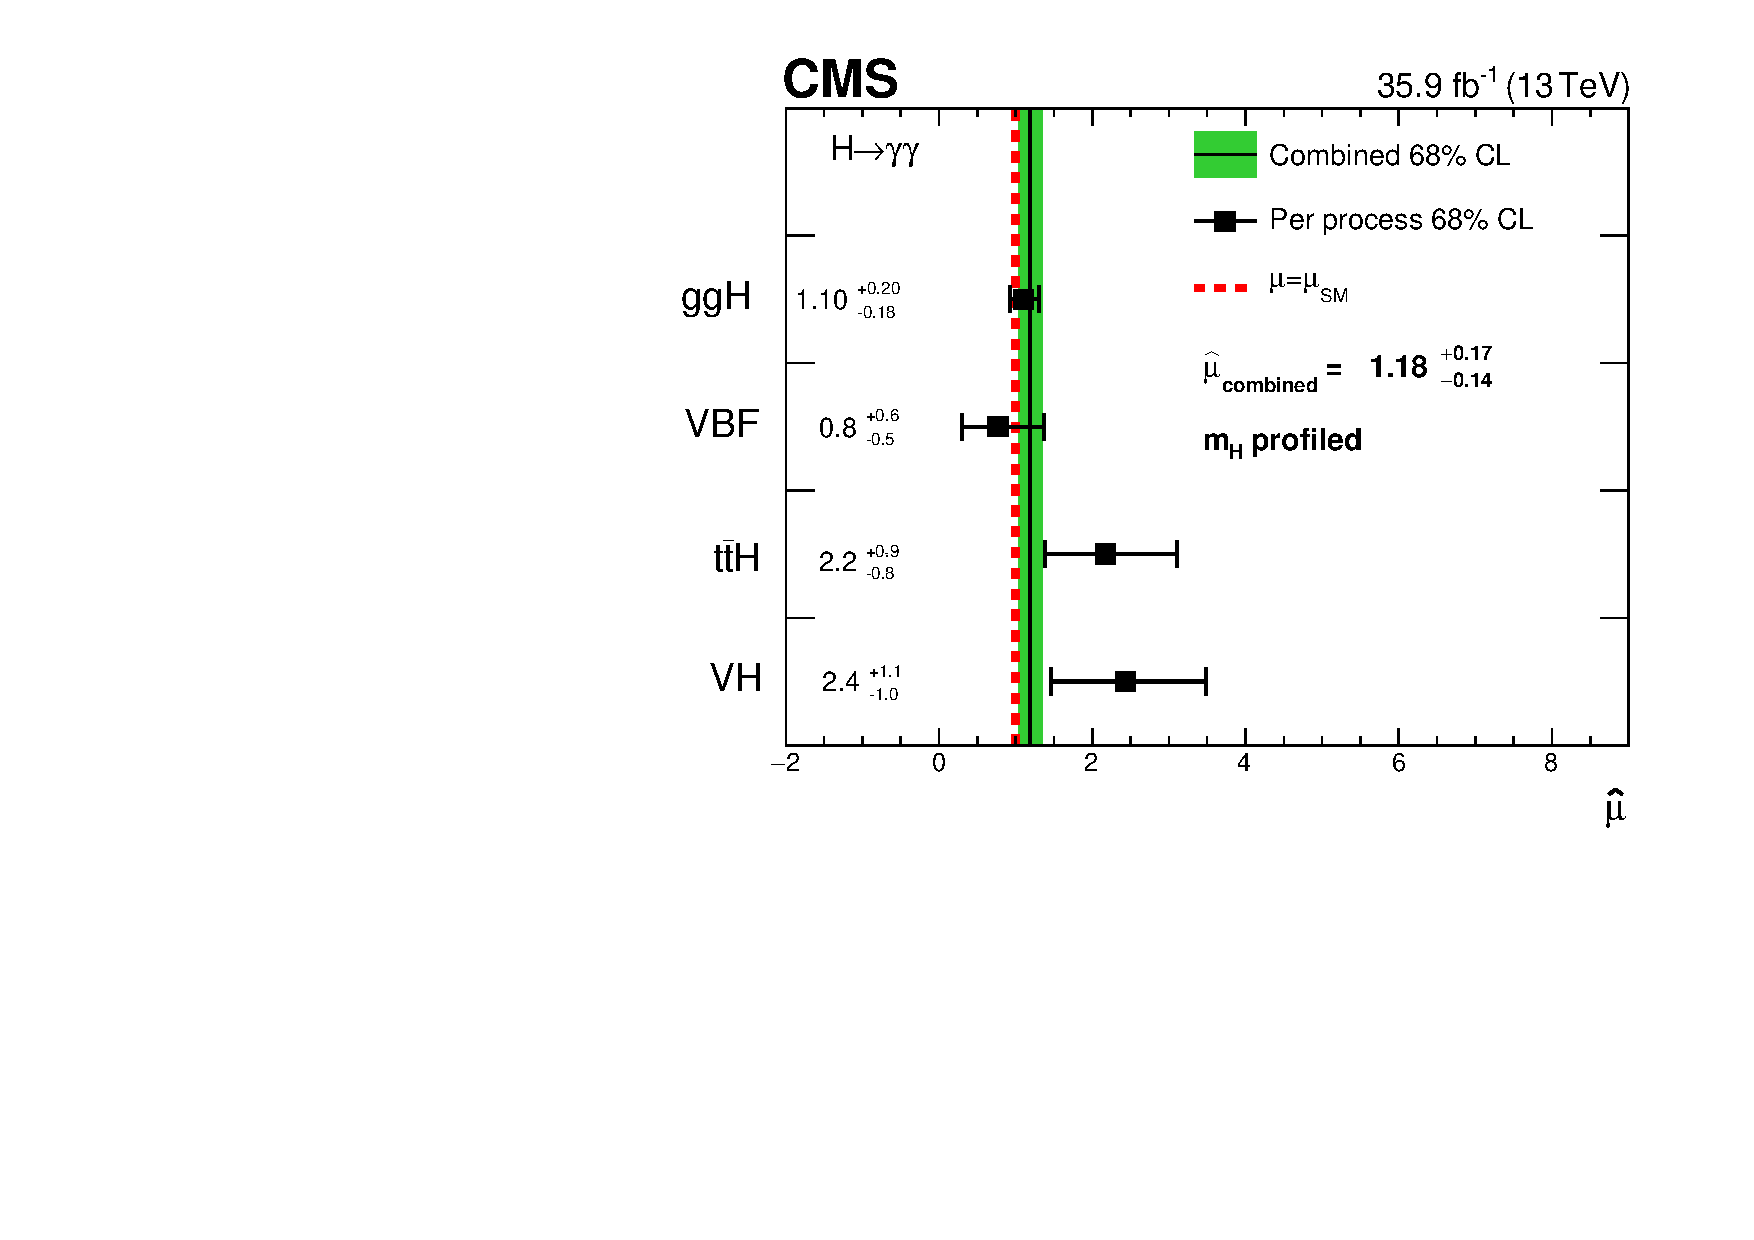
\includegraphics[width=0.9\textwidth]{Figures/Theory/PerProcTrad.pdf}
  \caption[Per process signal strength modifier measurements from Ref.~\cite{HIG-16-040}.]
  {
    Signal strength modifier measurements in the \Hgg decay channel.
    The modifiers for each process (black points) are shown, with the SM Higgs boson mass profiled, 
    compared to the overall signal strength modifier (green band) 
    and to the SM expectation (dashed red line).
    Figure first shown in Ref.~\cite{HIG-16-040}.
  }
  \label{fig:theory_PerProcTrad}
\end{figure}

\section{The simplified template cross section framework}

The simplified template cross section (STXS) framework \cite{YR4}
provides a coherent approach with which to perform precision Higgs boson measurements. 
Its goal is to minimise the theory-dependence of Higgs boson measurements, 
whilst permitting the use of advanced analysis techniques to optimise the measurements' sensitivities.
This also increases the reinterpretability of the measurements.
It is designed to supersede the traditional signal strength modifier measurements.

In the STXS framework, 
theoretically-motivated kinematic regions based upon Higgs boson production modes are defined.
These simplified regions, or bins, exist in varying degrees of granularity, 
following sequential ``stages".
Increasing the granularity of the signal bins 
provides additional information for different theoretical interpretations of the measurements, 
and enhances the sensitivity to possible signatures beyond the standard model.
As the integrated luminosity of the datasets collected by the LHC increases, 
so does the experimental sensitivity,
and measurements can progress to later stages within the STXS framework.

At the so-called STXS stage 0, 
the bins correspond closely to the different Higgs boson production mechanisms.
An additional requirement is placed on the Higgs boson rapidity $|y_H| < 2.5$, 
which reduces the theoretical uncertainty 
that would otherwise arise when extrapolating measurements to the full phase space,
a large part of which is not accessible experimentally.
The experimental acceptance of \Hgg events with $|y_H| > 2.5$ is negligible.
The stage 0 bins are illustrated in Figure~\ref{fig:theory_stage0}.
The principal difference from the production processes used in the signal strength measurements,
such as those shown in Figure~\ref{fig:theory_PerProcTrad},
is that VH production where the vector boson decays hadronically is grouped together with 
VBF production to define an ``electroweak qqH" bin.

\begin{figure}[hptb]
  \centering
  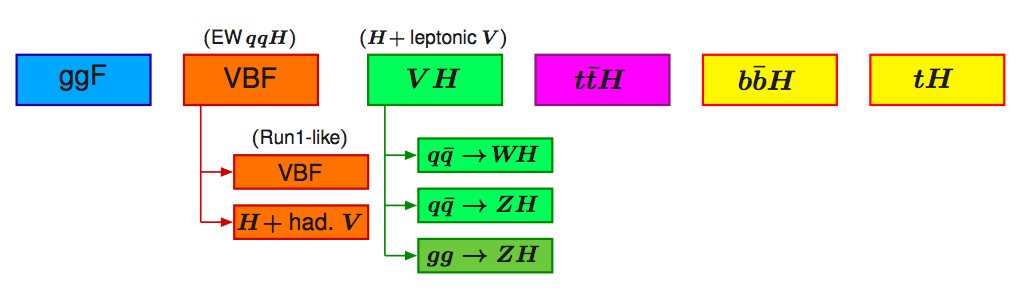
\includegraphics[width=\textwidth]{Figures/Theory/stage0.png}
  \caption[Stage 0 STXS bins.]
  {
    The STXS stage 0 bins. 
    The bins are designed to closely follow the Higgs boson production processes
    used for measurements during Run 1 of the LHC.
    Figure taken from Ref.~\cite{YR4}.
  }
  \label{fig:theory_stage0}
\end{figure}

Measurements of stage 0 cross sections in the \Hgg decay channel 
were performed in the previous CMS~\Hgg~analysis~\cite{HIG-16-040}.
The results are shown in Figure~\ref{fig:theory_PerProcSTXS}, 
which is similar to Figure~\ref{fig:theory_PerProcTrad}.
Aside from the change in signal bin definitions and the absence of an inclusive measurement, 
the main difference is in the treatment of the theoretical uncertainties.
When performing a measurement of $\mu$, 
a fit is performed for the signal strength modifier ratio $\sigma/\sigma_{\textrm{SM}}$. 
This requires that the theoretical uncertainty on the SM prediction, 
which enters via the denominator, be included.
In contrast if the fit parameter is just the observed cross section $\sigma$, 
the measurement does not depend on the overall SM prediction 
and this uncertainty does not need to be included.
It is instead considered as the uncertainty on the SM prediction, 
as displayed in Figure~\ref{fig:theory_PerProcSTXS}.
This separation of the theoretical uncertainties means that the measurement is less dependent 
on the theoretical prediction and remains useful 
even if improved theoretical predictions are obtained in the future.

\begin{figure}[hptb]
  \centering
  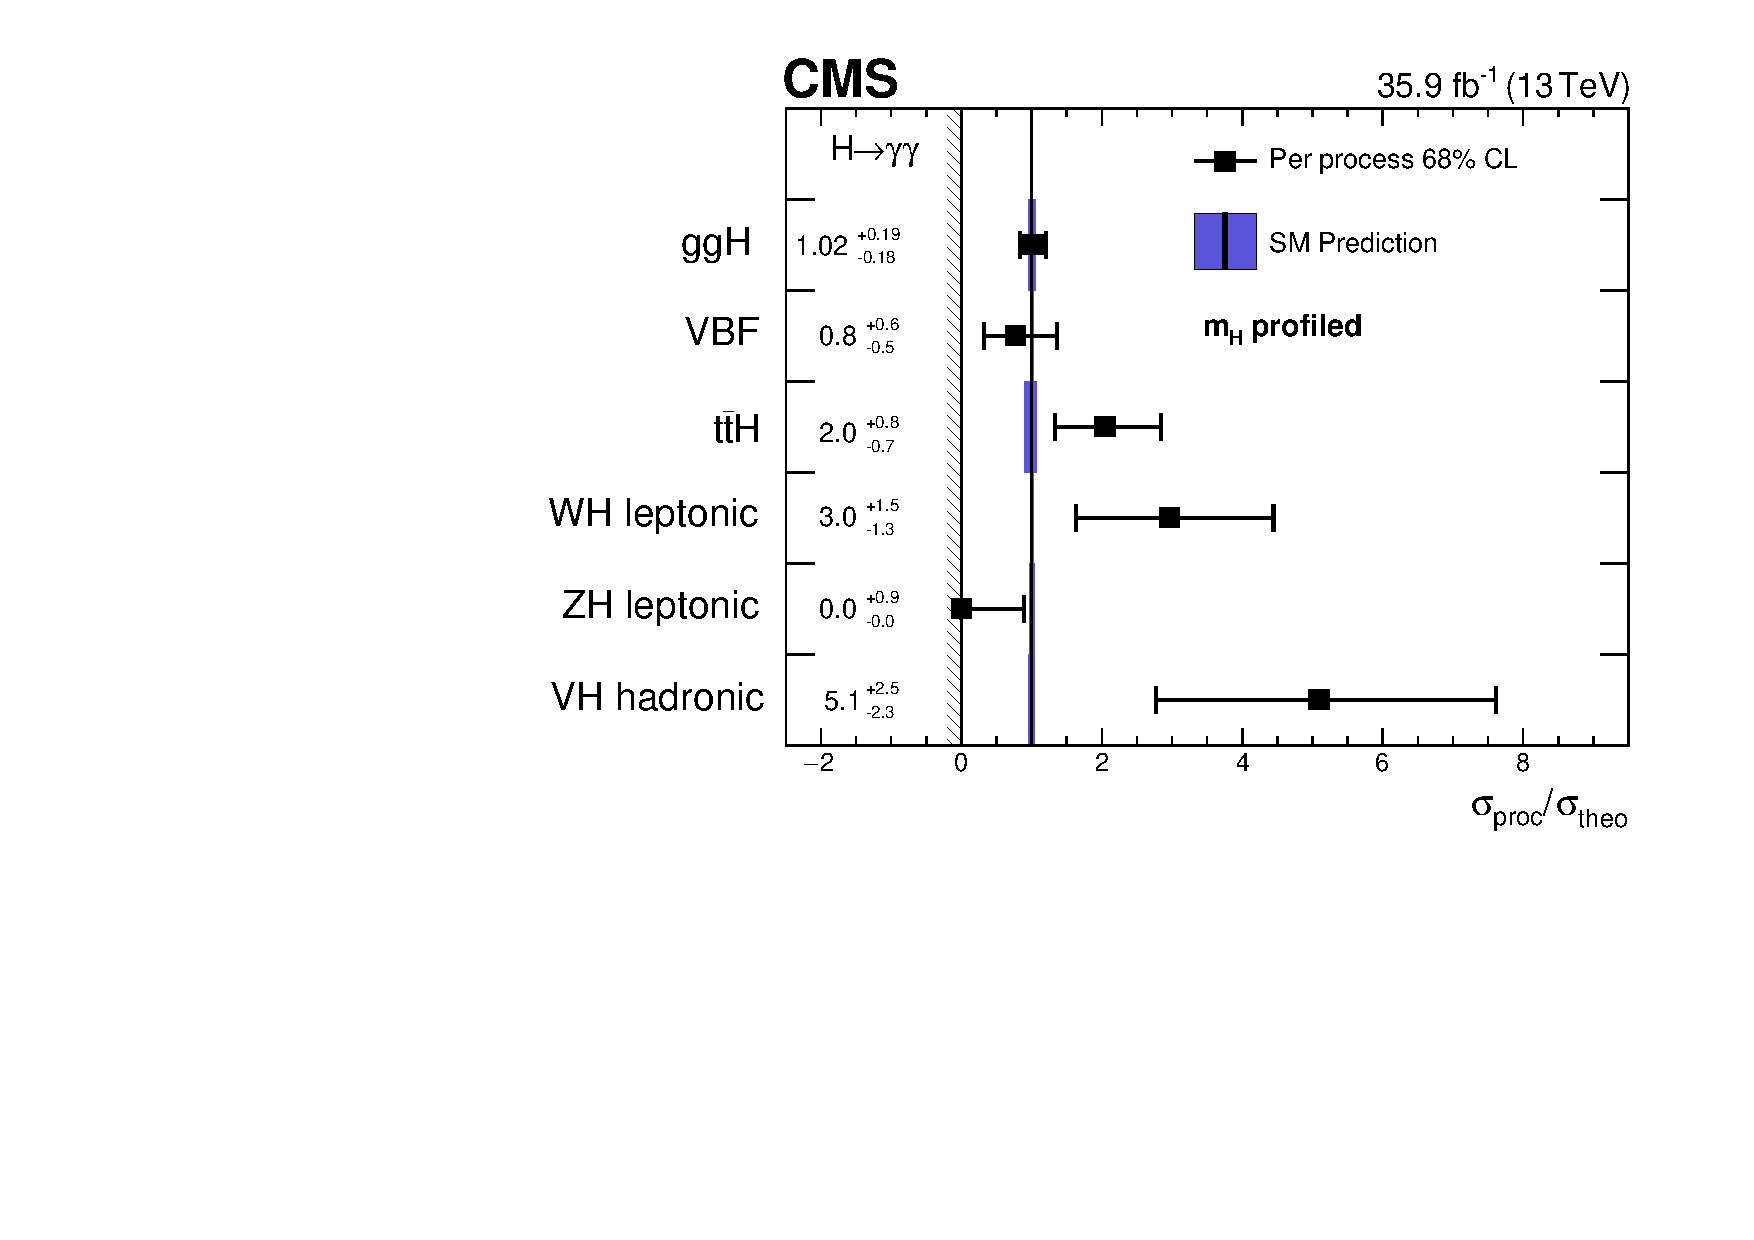
\includegraphics[width=0.9\textwidth]{Figures/Theory/PerProcSTXS.pdf}
  \caption[Stage 0 simplified template cross section measurements from Ref.~\cite{HIG-16-040}.]
  {
    Normalised cross sections measured for each stage 0 bin (black points) 
    in the STXS framework, 
    with the SM Higgs boson mass profiled, 
    compared to the SM expectations and their uncertainties (blue band). 
    The signal strength modifiers are constrained to be non-negative, 
    as indicated by the vertical line and hashed pattern at zero.
    Figure first shown in Ref.~\cite{HIG-16-040}.
  }
  \label{fig:theory_PerProcSTXS}
\end{figure}

At stage 1 of the STXS framework, 
a further splitting of bins into different kinematic regions is performed.
This provides additional information for different theoretical interpretations of the measurements, 
and enhances the sensitivity to possible signatures beyond the standard model.
Measurements at stage 1 of the framework have already been reported by the ATLAS Collaboration \cite{ATLAS_Hgg36,ATLAS_Hgg80,ATLASstage0_ZZ}; 
this analysis comprises the first CMS measurement of STXS stage 1 regions in the diphoton channel, 
covering the gluon fusion (ggH) and vector boson fusion (VBF) production modes.
The definitions of the different bins are shown in 
Figures~\ref{fig:theory_stage1ggH} and Figures~\ref{fig:theory_stage1VBF} 
for ggH and VBF production respectively.
For ggH production, bins are defined using the transverse momentum of the Higgs boson
and the number of jets in the event. 
In addition there are two bins for events with two jets where the event kinematics
resemble those of typical VBF events.
For VBF production, the bins are defined using the kinematics 
of the characteristic dijet system.
The ultimate goal of this analysis is to measure the cross sections of these bins 
as precisely as possible.
Further detail of the exact bin definitions 
and the methods used to discriminate between them is given in Chapter~\ref{chap:categorisation}.

\section{Summary}

The SM is a gauge field theory which describes all known fundamental particles 
and the forces which govern their interactions, with the exception of gravity.
Its predictions have been tested to extremely high levels of precision, 
and in 2012 the last remaining unobserved particle in the SM, the Higgs boson, was discovered.
The Higgs boson is a crucial piece of the SM as its existence is required to explain the origin
of the masses of both gauge bosons and fermions.
Once the mass of the Higgs boson, which has been measured experimentally, is known, 
its interactions with other particles in the SM are fully determined.
Performing precision measurements of the Higgs boson and its properties is therefore 
one of the foremost priorities in current particle physics research.
The STXS framework provides a coherent approach to performing 
these measurements, minimising the theoretical dependence of experimental results
whilst permitting the use of advanced analysis techniques.
This analysis aims to measure STXS bins in the \Hgg decay channel at various levels of granularity, 
thereby testing the SM and its predictions as stringently as possible.

\begin{figure}[hptb]
  \centering
  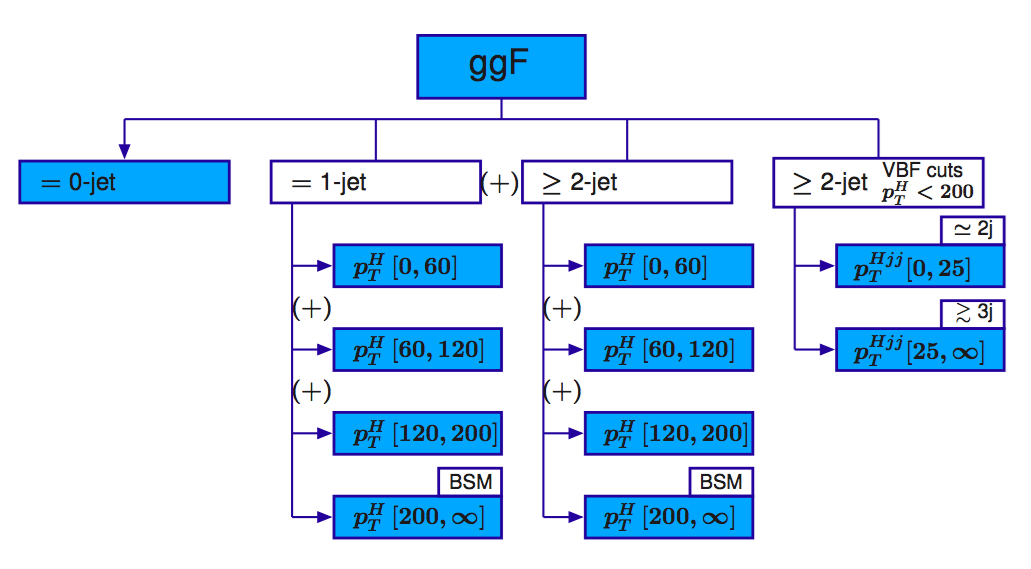
\includegraphics[width=\textwidth]{Figures/Theory/stage1ggH.png}
  \caption[Stage 1 STXS bins for the ggH production mode.]
  {
    The STXS stage 1 bins for the ggH production mode.
    The inclusive ggH process is subdivided into bins according to the transverse momentum 
    of the Higgs boson and the number of jets in the event.
    Figure taken from Ref.~\cite{YR4}.
  }
  \label{fig:theory_stage1ggH}
\end{figure}

\begin{figure}[hptb]
  \centering
  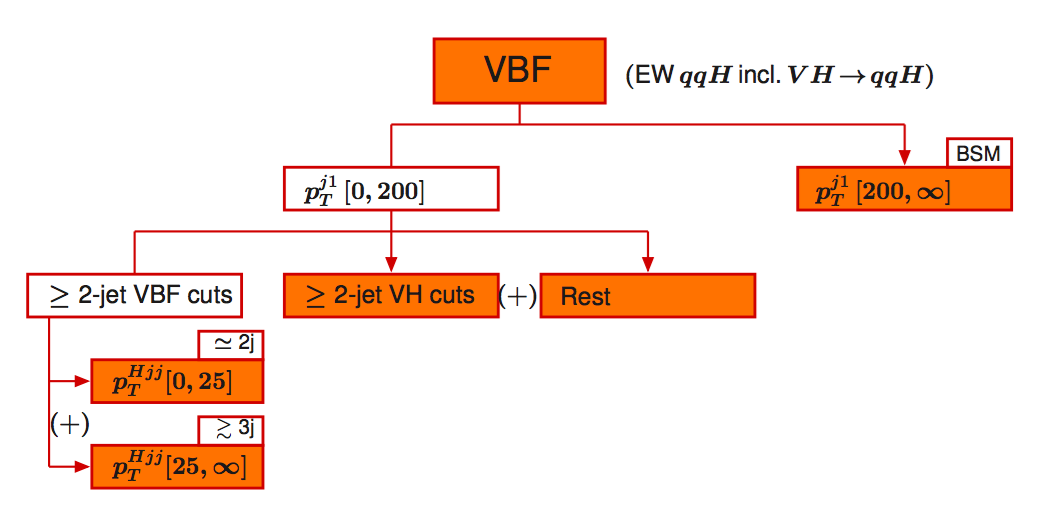
\includegraphics[width=\textwidth]{Figures/Theory/stage1VBF.png}
  \caption[Stage 1 STXS bins for the VBF production mode.]
  {
    The STXS stage 1 bins for the VBF production mode.
    Both VBF events and VH events where the vector boson decays hadronically are included.
    The inclusive processes are subdivided according to the kinematics of the Higgs boson 
    and the jets in the event.
    Figure taken from Ref.~\cite{YR4}.
  }
  \label{fig:theory_stage1VBF}
\end{figure}
